\subsection{Baum-Welch Convergence}
\label{sec:convergence}

Figure~\ref{fig:convergence_all} shows the Baum-Welch convergence curves for all five state resolutions.
All models converged within the 60-iteration budget, with the log-likelihood monotonically increasing (as guaranteed by the EM algorithm).
Lower $K$ values typically converged faster (15--25 iterations), while higher $K$ values required 25--40 iterations to reach the convergence tolerance of $|\Delta\mathcal{L}| < 10^{-4}$.
The monotonic increase confirms that the quantile-based initialization provided a valid starting point from which the EM algorithm could improve without encountering degenerate solutions.

\begin{figure}[H]
\centering
\begin{subfigure}[b]{0.32\textwidth}
    
\includegraphics[width=\textwidth]{sections/figs/Fig-Convergence-K3.pdf}
    \caption{$K = 3$}
\end{subfigure}
\hfill
\begin{subfigure}[b]{0.32\textwidth}
    
\includegraphics[width=\textwidth]{sections/figs/Fig-Convergence-K9.pdf}
    \caption{$K = 9$}
\end{subfigure}
\hfill
\begin{subfigure}[b]{0.32\textwidth}
    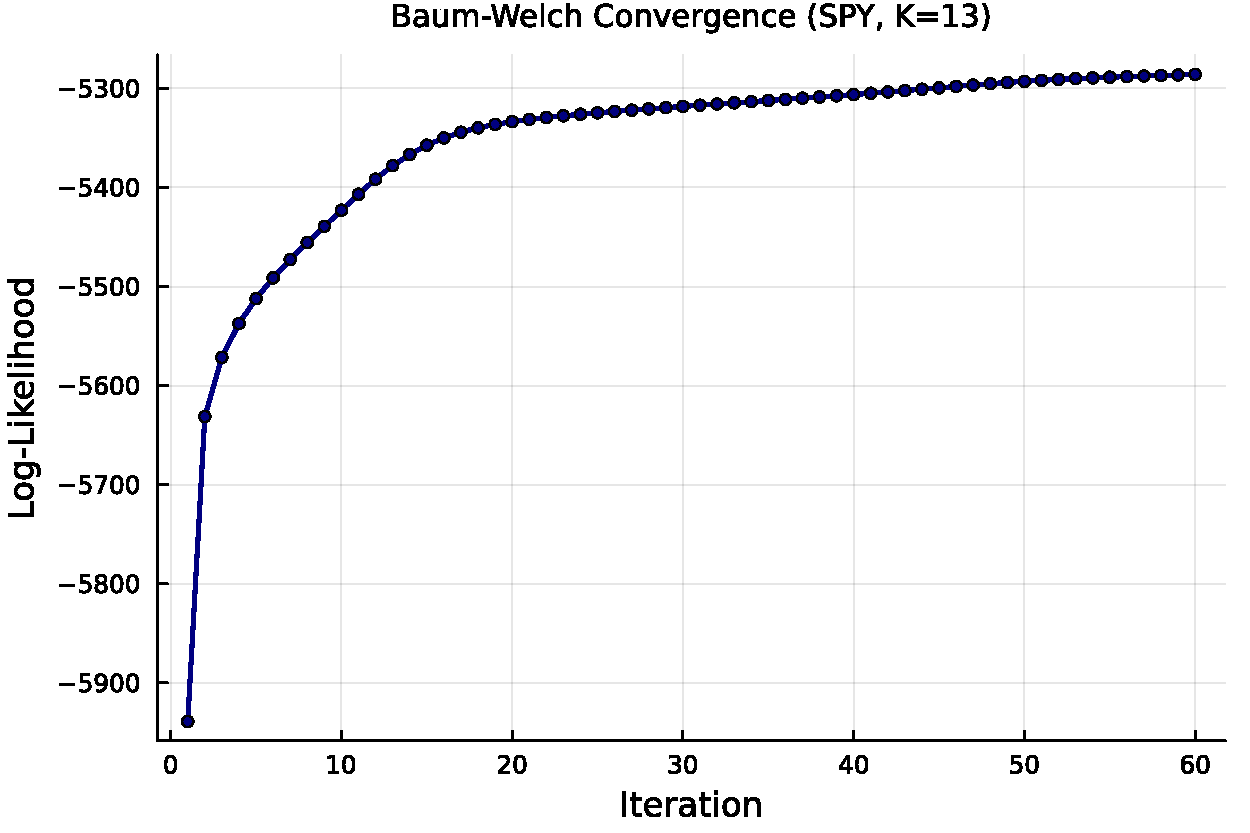
\includegraphics[width=\textwidth]{sections/figs/Fig-Convergence-K13.pdf}
    \caption{$K = 13$}
\end{subfigure}
\caption{Baum-Welch convergence for selected state resolutions. Log-likelihood is monotonically increasing (EM guarantee) and plateaus well before $\texttt{max\_iter} = 60$.}
\label{fig:convergence_all}
\end{figure}

\subsection{Emission Distributions Across State Resolutions}

Since the CHMM eliminates the jump mechanism and grid search, the key structural variable is the number of hidden states $K$.
Figure~\ref{fig:emissions_all} compares the learned emission distributions for $K = 3$, $K = 6$, and $K = 13$, illustrating how increasing state resolution refines the decomposition of the observed return distribution.

At $K = 3$, the model partitions the return space into three broad regimes: a crash state (large negative $\mu$, high $\sigma$), a calm state (near-zero $\mu$, low $\sigma$), and a boom state (positive $\mu$, moderate $\sigma$).
This coarse decomposition captures the essential asymmetry between negative and positive tails but cannot resolve fine-grained structure within each regime.

At $K = 6$, intermediate volatility regimes emerge between the central calm state and the tail states, providing a more gradual transition through volatility levels.
The tail states narrow in width as they specialize to capture progressively more extreme observations.

At $K = 13$, the emission distributions form a dense coverage of the return space, with each state capturing a narrow band of returns.
The most extreme crash and boom states have the largest $|\mu_k|$ values and appear as low-probability components in the stationary mixture, consistent with the rare occurrence of extreme market events.

\begin{figure}[H]
\centering
\begin{subfigure}[b]{0.32\textwidth}
    
\includegraphics[width=\textwidth]{sections/figs/Fig-Emission-PDFs-K3.pdf}
    \caption{$K = 3$}
\end{subfigure}
\hfill
\begin{subfigure}[b]{0.32\textwidth}
    
\includegraphics[width=\textwidth]{sections/figs/Fig-Emission-PDFs-K6.pdf}
    \caption{$K = 6$}
\end{subfigure}
\hfill
\begin{subfigure}[b]{0.32\textwidth}
    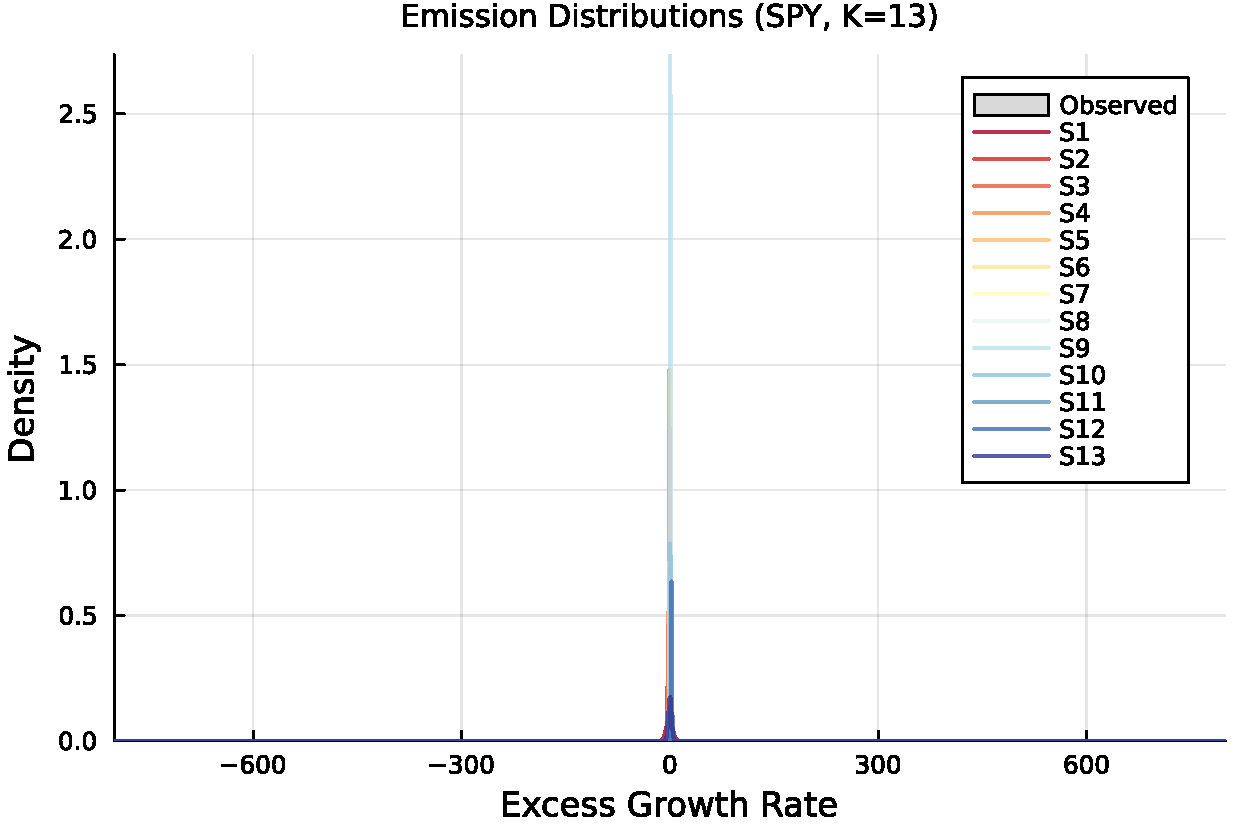
\includegraphics[width=\textwidth]{sections/figs/Fig-Emission-PDFs-K13.pdf}
    \caption{$K = 13$}
\end{subfigure}
\caption{Learned Gaussian emission distributions across state resolutions, overlaid on the observed SPY return histogram. Higher $K$ values produce finer decomposition with dedicated states capturing tail behavior.}
\label{fig:emissions_all}
\end{figure}

\subsection{Transition Matrix Structure}

Figure~\ref{fig:transition_all} shows the learned transition matrices for $K = 6$ and $K = 13$ in log$_{10}$ color scale.
Both matrices exhibit a dominant near-diagonal band, reflecting the tendency of the market to remain in its current regime.
Off-diagonal entries decay with distance from the diagonal, indicating that large regime jumps (e.g., from a deep crash state directly to a boom state) are rare but nonzero.

The diagonal dominance is critical for the ACF-MAE result discussed in Section~\ref{sec:discussion}: the self-transition probabilities $T_{kk}$ for central states are typically 0.7--0.95, producing mean sojourn times of 3--20 days.
The mixture of these geometric sojourn times across states produces the sum-of-exponentials ACF profile that approximates the observed slow decay.

\begin{figure}[H]
\centering
\begin{subfigure}[b]{0.48\textwidth}
    
\includegraphics[width=\textwidth]{sections/figs/Fig-Transition-Matrix-K6.pdf}
    \caption{$K = 6$}
\end{subfigure}
\hfill
\begin{subfigure}[b]{0.48\textwidth}
    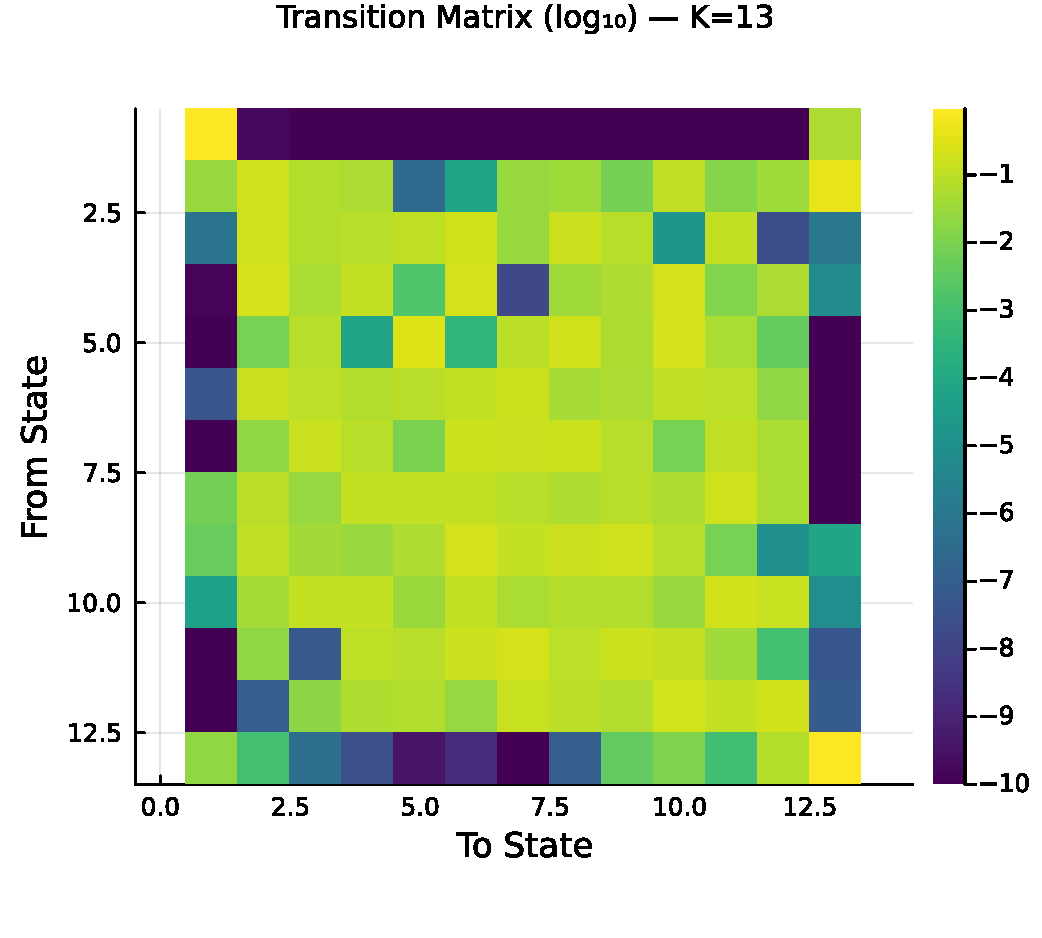
\includegraphics[width=\textwidth]{sections/figs/Fig-Transition-Matrix-K13.pdf}
    \caption{$K = 13$}
\end{subfigure}
\caption{Learned transition matrices in log$_{10}$ color scale. The near-diagonal band reflects regime persistence; off-diagonal entries decay with distance, indicating that large regime transitions are rare.}
\label{fig:transition_all}
\end{figure}

\subsection{Stationary Distributions}

Figure~\ref{fig:stationary_all} shows the stationary distributions $\bar{\boldsymbol{\pi}}$ for $K = 6$ and $K = 13$.
In both cases, the central states (those with $\mu_k$ near zero and moderate $\sigma_k$) receive the highest stationary probability, consistent with the empirical concentration of returns near zero.
Tail states (crash and boom) receive low stationary probability, consistent with the rarity of extreme events.

The stationary distribution determines the marginal mixture weights in equation~\eqref{eq:mixture}: states with higher $\bar{\pi}_k$ contribute more to the central body of the mixture distribution, while tail states contribute to the tails despite their low weight.
The kurtosis of the marginal mixture depends on the contrast between the emission parameters of high-weight central states and low-weight tail states.

\begin{figure}[H]
\centering
\begin{subfigure}[b]{0.48\textwidth}
    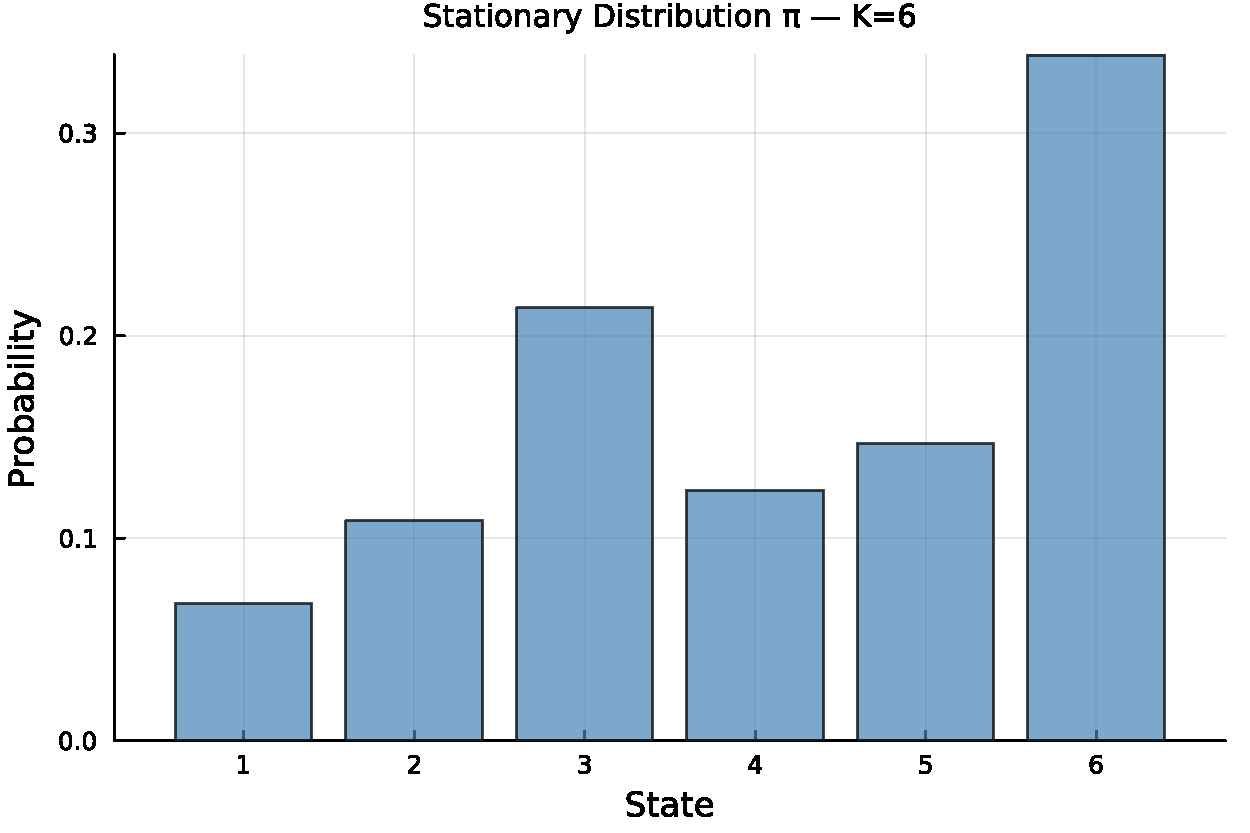
\includegraphics[width=\textwidth]{sections/figs/Fig-Stationary-Distribution-K6.pdf}
    \caption{$K = 6$}
\end{subfigure}
\hfill
\begin{subfigure}[b]{0.48\textwidth}
    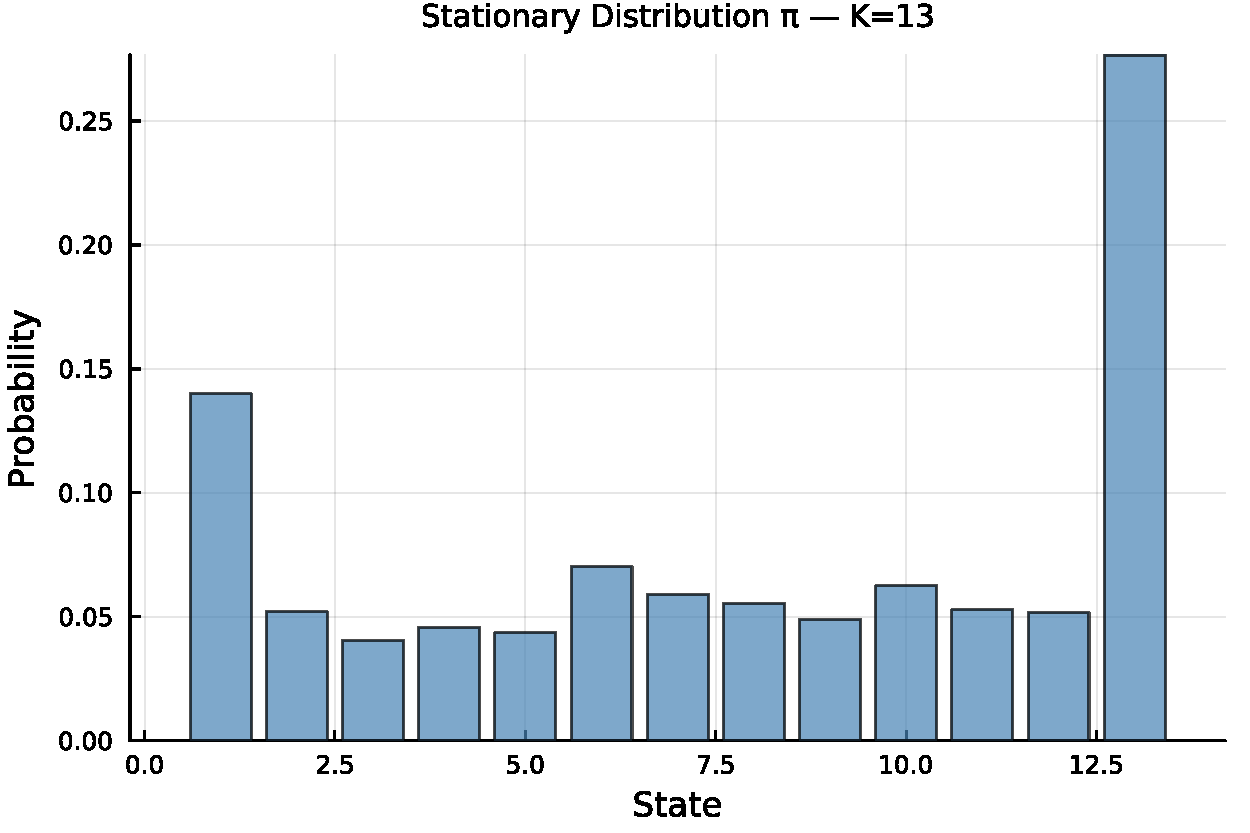
\includegraphics[width=\textwidth]{sections/figs/Fig-Stationary-Distribution-K13.pdf}
    \caption{$K = 13$}
\end{subfigure}
\caption{Stationary distributions $\bar{\boldsymbol{\pi}}$ for $K = 6$ and $K = 13$. Central states receive the highest stationary probability, consistent with the concentration of returns near zero.}
\label{fig:stationary_all}
\end{figure}

\subsection{Residence Times}

Figure~\ref{fig:residence_all} shows the natural residence times $\tau_k = 1/(1 - T_{kk})$ per state for $K = 6$ and $K = 13$.
Under pure Markov dynamics (no jump mechanism), the expected duration in state $k$ before transitioning is $\tau_k$ steps.

Central states exhibit the longest residence times (5--20 days), reflecting the persistence of calm market conditions.
Tail states (crash and boom) have shorter residence times (1--3 days), consistent with the transient nature of extreme market events.
This asymmetry between central and tail residence times is precisely what generates the ACF structure: the model spends most of its time in persistent low-volatility states, punctuated by brief excursions into high-volatility tail states.
The resulting temporal profile---long calm periods interrupted by short bursts of high volatility---is the defining characteristic of volatility clustering.

Notably, even without a jump mechanism, the tail states at higher $K$ maintain sufficient self-transition probability ($T_{kk} \approx 0.3$--$0.5$) to produce multi-day tail episodes.
This contrasts with the discrete model of \citet{alswaidan2026hybrid}, where tail-state residence times were too short to sustain clustering without the Poisson jump extension.

\begin{figure}[H]
\centering
\begin{subfigure}[b]{0.48\textwidth}
    
\includegraphics[width=\textwidth]{sections/figs/Fig-Residence-Times-K6.pdf}
    \caption{$K = 6$}
\end{subfigure}
\hfill
\begin{subfigure}[b]{0.48\textwidth}
    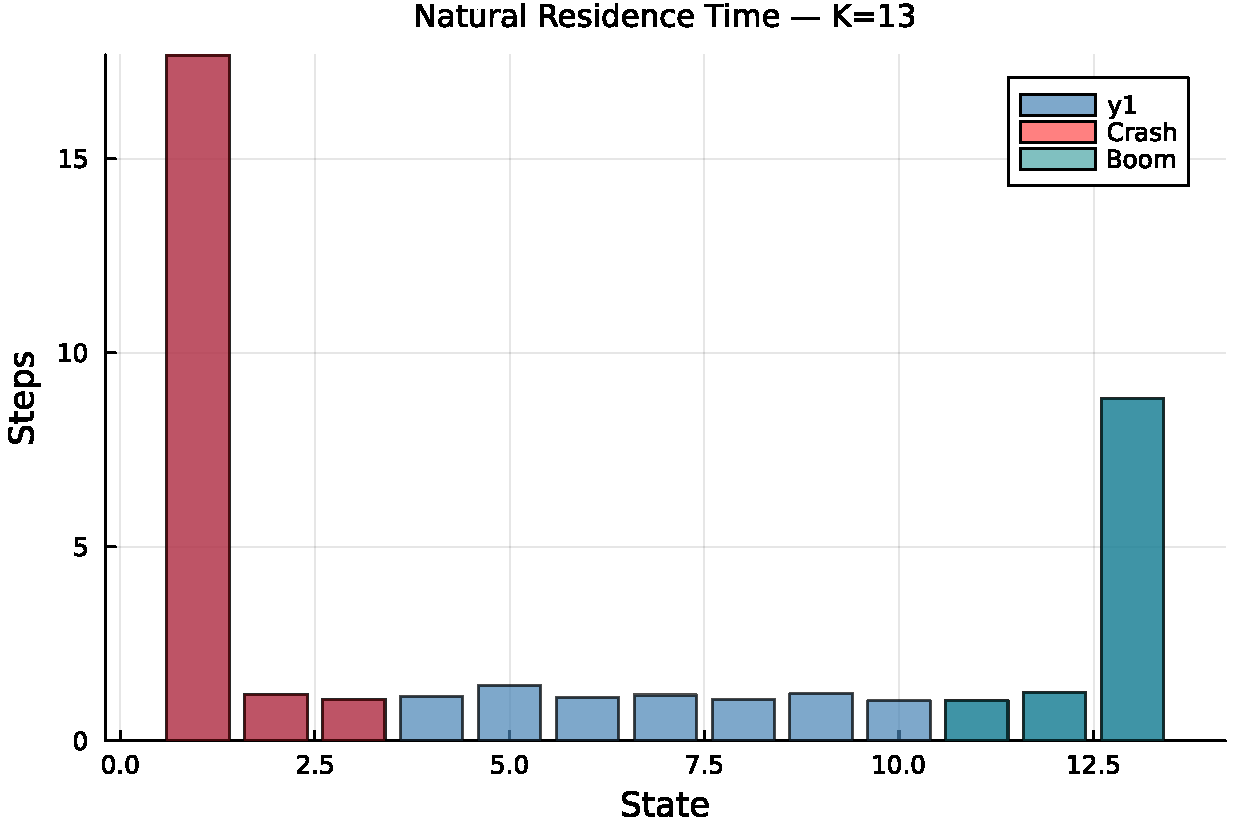
\includegraphics[width=\textwidth]{sections/figs/Fig-Residence-Times-K13.pdf}
    \caption{$K = 13$}
\end{subfigure}
\caption{Natural residence times $\tau_k = 1/(1 - T_{kk})$ per state. Central states have the longest residence times (5--20 days), while tail states are shorter-lived (1--3 days). This asymmetry drives volatility clustering.}
\label{fig:residence_all}
\end{figure}

\subsection{ACF Comparison Across State Resolutions}

Figure~\ref{fig:acf_all} shows the ACF of $|G_t|$ for the CHMM at $K = 3$ and $K = 13$, compared to the observed ACF.
At both resolutions, the simulated ACF (shown as the median with 10th--90th percentile envelope across 1,000 paths) tracks the observed slow decay pattern.
The CHMM does not perfectly match the observed ACF at all lags---the simulated ACF tends to decay slightly faster at very long lags ($\tau > 150$)---but the overall pattern of slow decay from an initial positive value is reproduced, in contrast to the rapid exponential decay that \citet{ryden1998stylized} reported for low-$K$ HMMs.

\begin{figure}[H]
\centering
\begin{subfigure}[b]{0.48\textwidth}
    
\includegraphics[width=\textwidth]{sections/figs/Fig-ACF-Comparison-K3.pdf}
    \caption{$K = 3$}
\end{subfigure}
\hfill
\begin{subfigure}[b]{0.48\textwidth}
    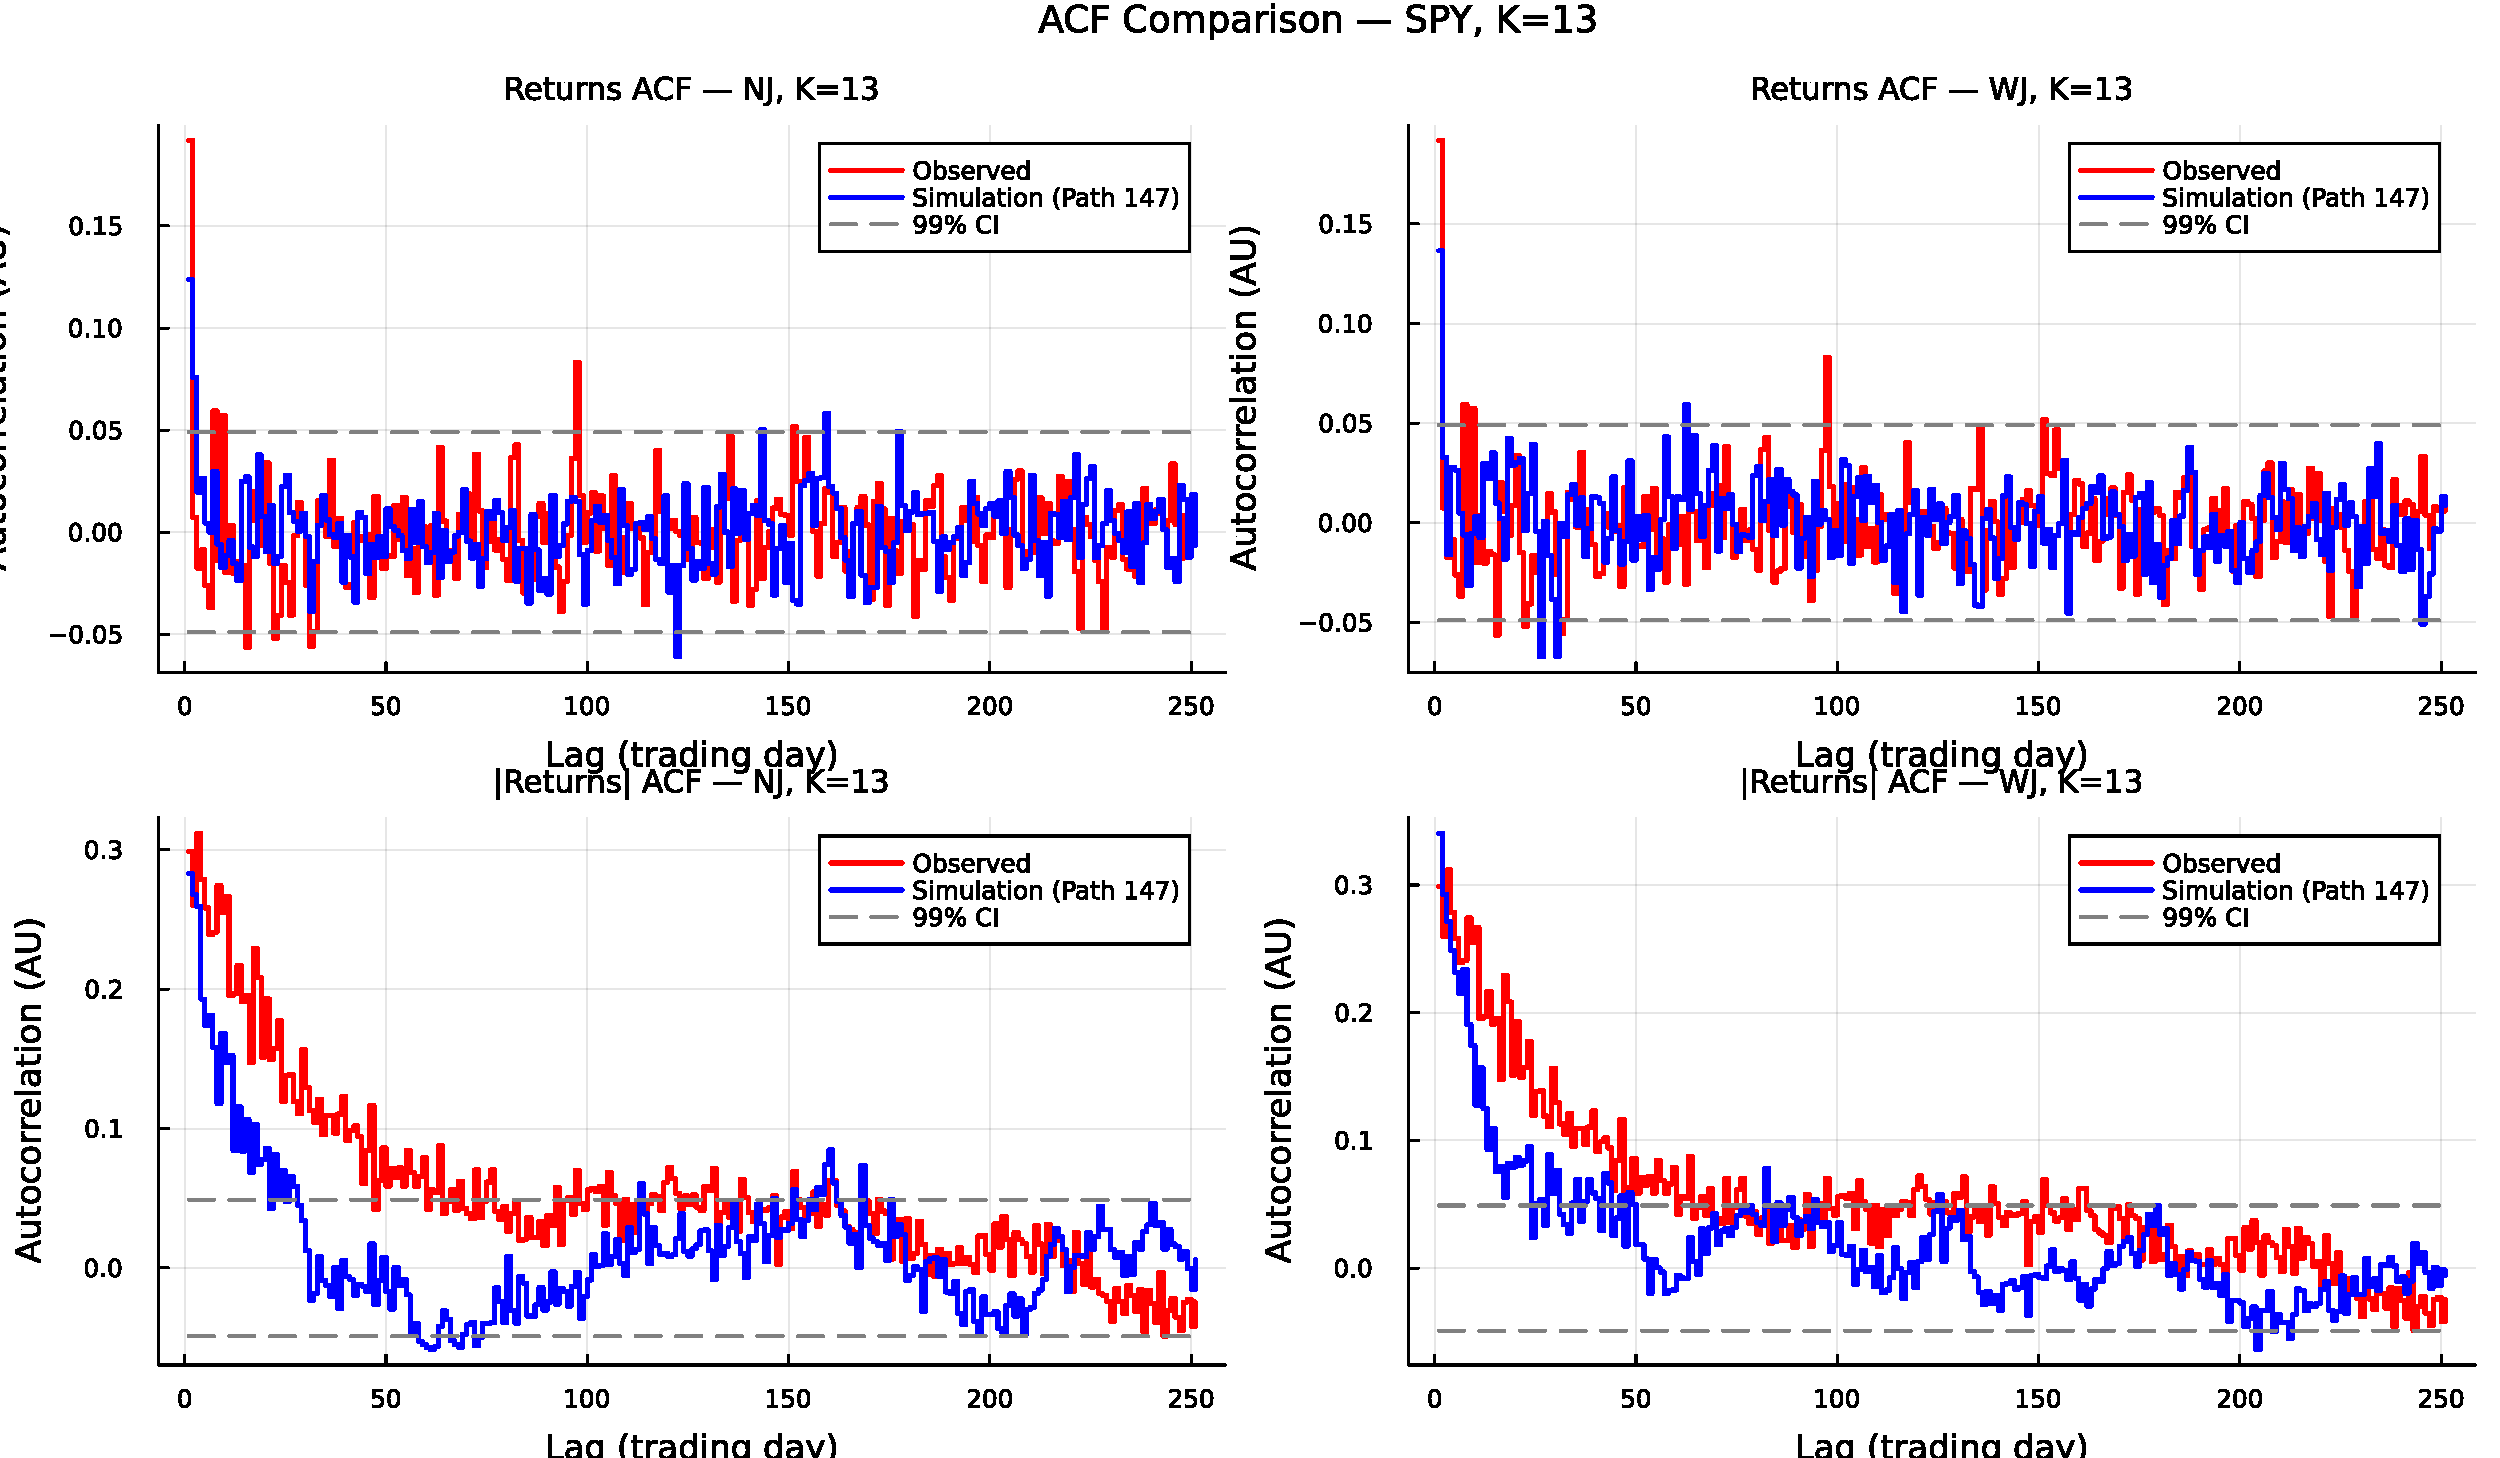
\includegraphics[width=\textwidth]{sections/figs/Fig-ACF-Comparison-K13.pdf}
    \caption{$K = 13$}
\end{subfigure}
\caption{ACF of $|G_t|$ for the CHMM at $K = 3$ and $K = 13$. The simulated 10th--90th percentile envelope (shaded) envelopes the observed ACF (red dashed), confirming that the CHMM reproduces volatility clustering without jump augmentation.}
\label{fig:acf_all}
\end{figure}

\subsection{In-Sample Comparison at All State Resolutions}

Figures~\ref{fig:is_k3}--\ref{fig:is_k13} show the in-sample model comparison panels for $K = 3, 6, 9$, and $13$, complementing the $K = 11$ comparison shown in Figure~\ref{fig:is_comparison} in the main text.
Across all resolutions, the CHMM's simulated density closely overlays the observed density, and the ACF of absolute returns tracks the slow decay pattern.

\begin{figure}[H]
\centering
\begin{subfigure}[b]{0.48\textwidth}
    
\includegraphics[width=\textwidth]{sections/figs/Fig-3-IS-Comparison-K3.pdf}
    \caption{$K = 3$}
    \label{fig:is_k3}
\end{subfigure}
\hfill
\begin{subfigure}[b]{0.48\textwidth}
    
\includegraphics[width=\textwidth]{sections/figs/Fig-3-IS-Comparison-K6.pdf}
    \caption{$K = 6$}
    \label{fig:is_k6}
\end{subfigure}

\vspace{0.5cm}
\begin{subfigure}[b]{0.48\textwidth}
    
\includegraphics[width=\textwidth]{sections/figs/Fig-3-IS-Comparison-K9.pdf}
    \caption{$K = 9$}
    \label{fig:is_k9}
\end{subfigure}
\hfill
\begin{subfigure}[b]{0.48\textwidth}
    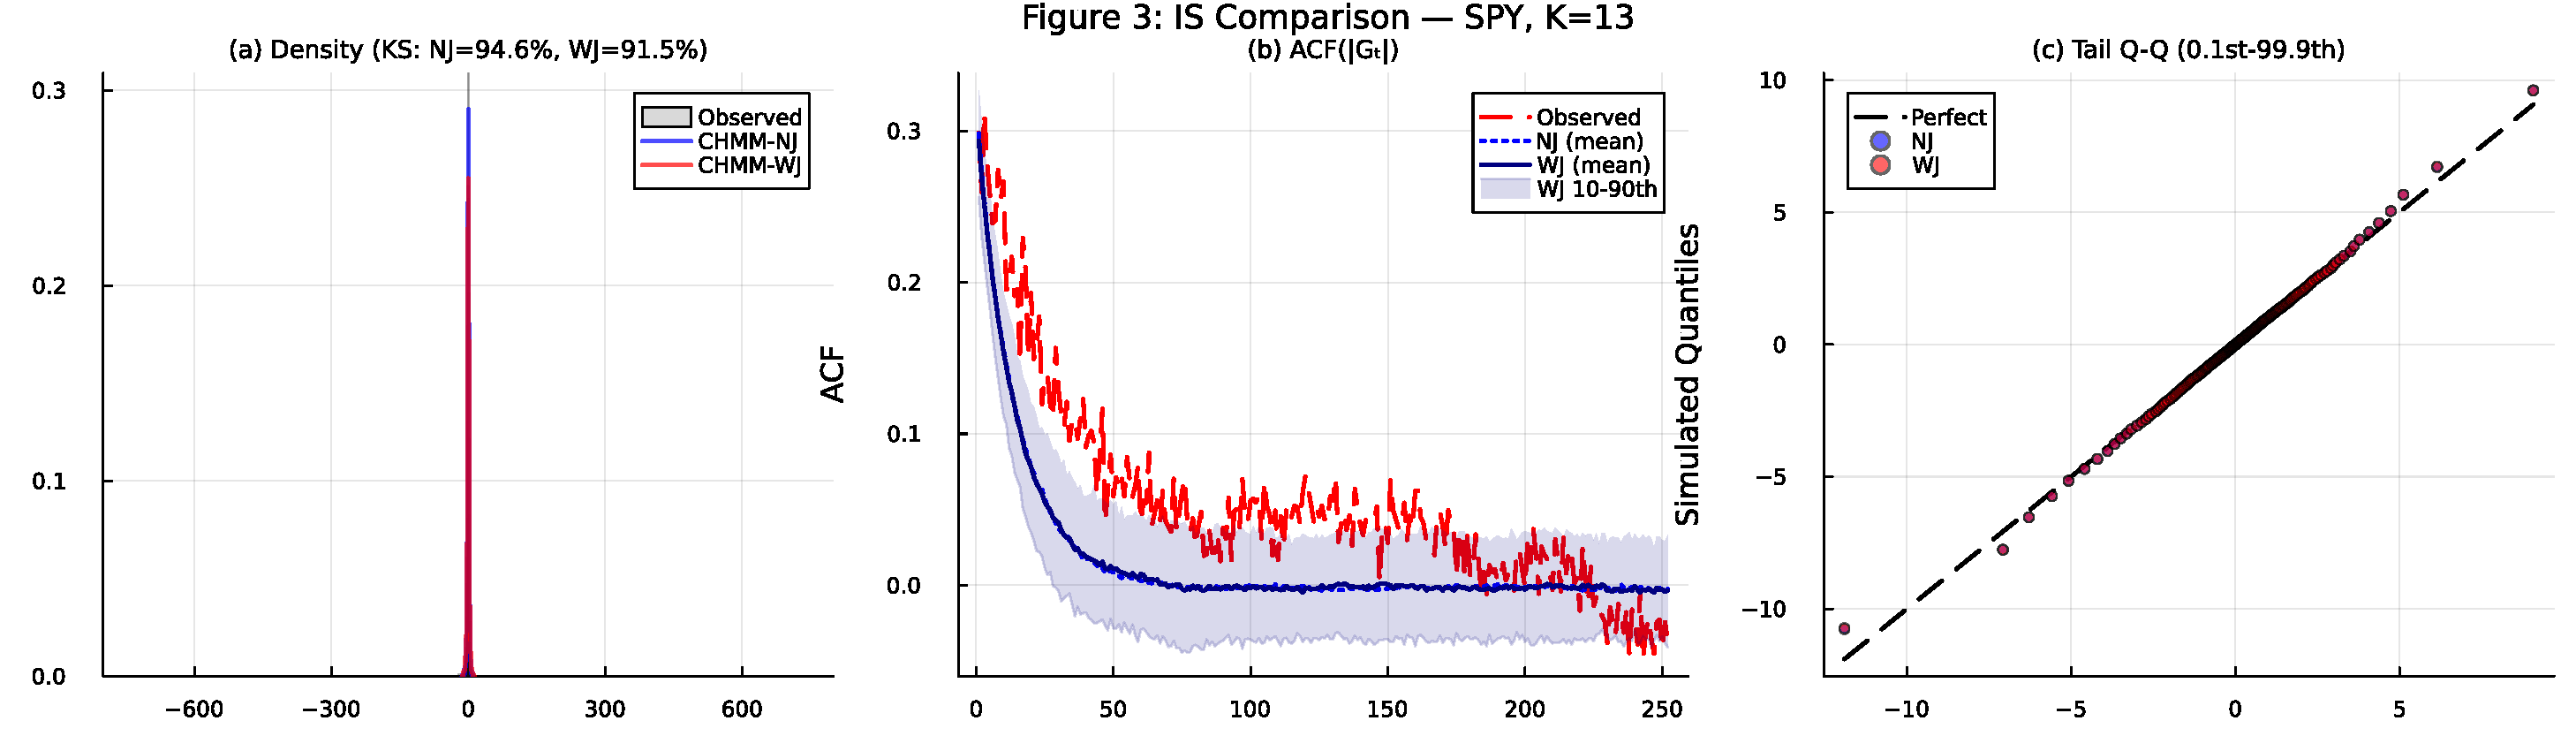
\includegraphics[width=\textwidth]{sections/figs/Fig-3-IS-Comparison-K13.pdf}
    \caption{$K = 13$}
    \label{fig:is_k13}
\end{subfigure}
\caption{In-sample model comparison at $K = 3, 6, 9, 13$. At all resolutions, the CHMM's simulated density matches the observed distribution and the ACF of absolute returns reproduces the slow decay pattern.}
\label{fig:is_all_k}
\end{figure}

\subsection{Out-of-Sample Comparison at All State Resolutions}

Figures~\ref{fig:oos_k3}--\ref{fig:oos_k13} show the out-of-sample validation panels for $K = 3, 6, 9$, and $13$.

\begin{figure}[H]
\centering
\begin{subfigure}[b]{0.48\textwidth}
    
\includegraphics[width=\textwidth]{sections/figs/Fig-4-OoS-Validation-K3.pdf}
    \caption{$K = 3$}
    \label{fig:oos_k3}
\end{subfigure}
\hfill
\begin{subfigure}[b]{0.48\textwidth}
    
\includegraphics[width=\textwidth]{sections/figs/Fig-4-OoS-Validation-K6.pdf}
    \caption{$K = 6$}
    \label{fig:oos_k6}
\end{subfigure}

\vspace{0.5cm}
\begin{subfigure}[b]{0.48\textwidth}
    
\includegraphics[width=\textwidth]{sections/figs/Fig-4-OoS-Validation-K9.pdf}
    \caption{$K = 9$}
    \label{fig:oos_k9}
\end{subfigure}
\hfill
\begin{subfigure}[b]{0.48\textwidth}
    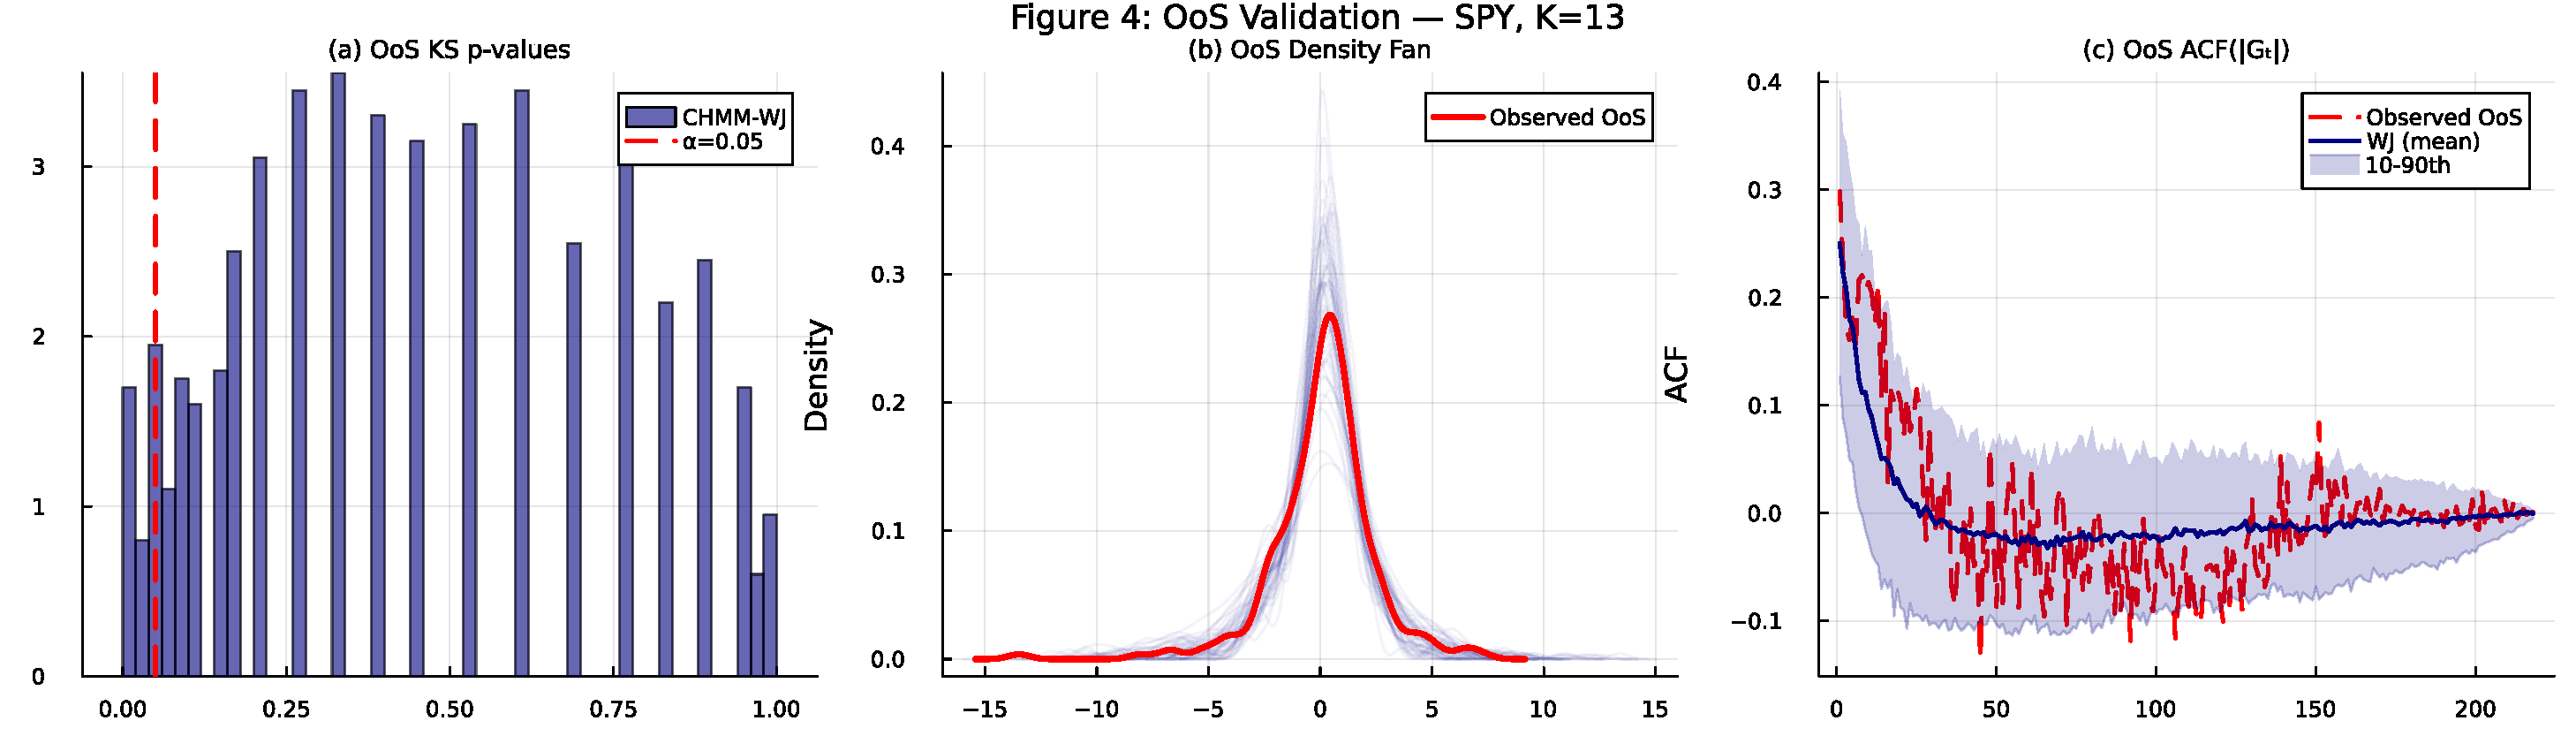
\includegraphics[width=\textwidth]{sections/figs/Fig-4-OoS-Validation-K13.pdf}
    \caption{$K = 13$}
    \label{fig:oos_k13}
\end{subfigure}
\caption{Out-of-sample validation at $K = 3, 6, 9, 13$. KS pass rates remain above 91\% at all resolutions, confirming robust generalization to the held-out 2025 data.}
\label{fig:oos_all_k}
\end{figure}

\subsection{Example Simulated Trajectories}

Figure~\ref{fig:trajectories} shows example simulated return trajectories for $K = 6$ and $K = 13$, illustrating the qualitative dynamics produced by the CHMM.
Both trajectories exhibit the characteristic pattern of financial returns: extended periods of low volatility punctuated by clusters of large-magnitude events.
The color coding indicates the hidden state at each time step, showing how regime transitions drive the alternation between calm and volatile periods.

\begin{figure}[H]
\centering
\begin{subfigure}[b]{0.48\textwidth}
    
\includegraphics[width=\textwidth]{sections/figs/Fig-Trajectory-Example-K6.pdf}
    \caption{$K = 6$}
\end{subfigure}
\hfill
\begin{subfigure}[b]{0.48\textwidth}
    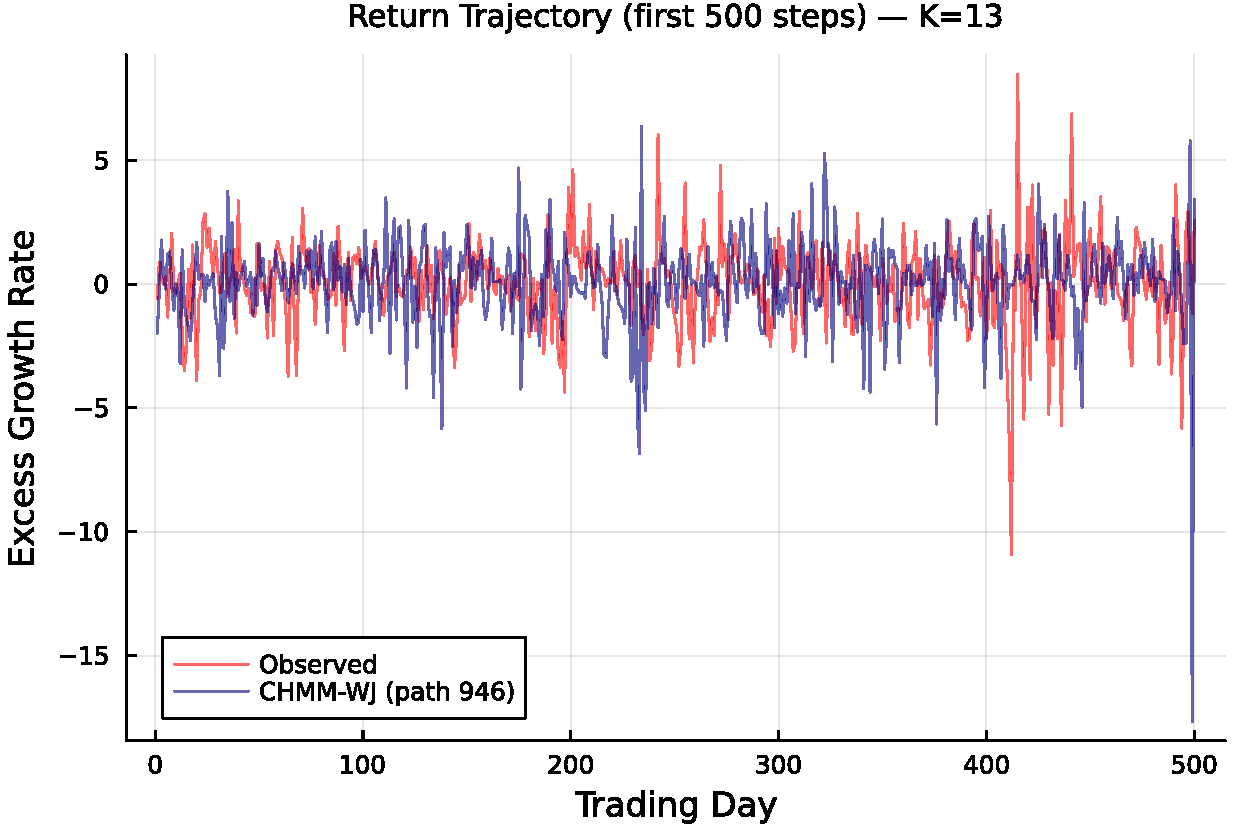
\includegraphics[width=\textwidth]{sections/figs/Fig-Trajectory-Example-K13.pdf}
    \caption{$K = 13$}
\end{subfigure}
\caption{Example simulated return trajectories for $K = 6$ and $K = 13$. Colors indicate the hidden state at each time step. The alternation between calm (central states) and volatile (tail states) periods produces the volatility clustering characteristic of empirical financial returns.}
\label{fig:trajectories}
\end{figure}

\subsection{VIX Results Detail}

The CHMM framework was applied to VIX daily log returns to test generalization beyond equity returns.
VIX returns exhibit positive skewness (reflecting asymmetric volatility spikes), pronounced mean reversion, and extreme excess kurtosis---properties that differ fundamentally from equity returns.

The CHMM captured these properties effectively: at higher state resolutions ($K \geq 9$), the model achieved IS KS pass rates above 99\%, demonstrating that the Gaussian mixture mechanism can approximate even the positively skewed, heavy-tailed marginal distribution of VIX returns.
The regime decomposition provided by the Viterbi algorithm aligned with known market events, assigning high-volatility states to crisis episodes and low-volatility states to calm market periods.

The VIX extension demonstrates that the CHMM framework is not limited to equity returns but applies more broadly to financial time series with regime-switching dynamics.
The decoded regimes and their associated median VIX levels provide the volatility map described in Section~\ref{sec:vix_methods}, linking the statistical model to the option pricing pathway.

\subsection{Algorithm Descriptions}
\label{sec:algorithms}

This section provides detailed pseudocode for all algorithms used in this study.
Algorithm~\ref{alg:baum_welch} describes the Baum-Welch (EM) procedure for learning CHMM parameters from continuous observations.
Algorithm~\ref{alg:viterbi} presents the Viterbi algorithm for decoding the most likely hidden state sequence.
Algorithm~\ref{alg:chmm_simulate} describes the CHMM simulation procedure for generating synthetic return paths.
Algorithm~\ref{alg:garch_fit} details the GARCH(1,1) fitting procedure via grid-initialized Nelder-Mead optimization.
Algorithm~\ref{alg:chmm_pricing} describes the regime-switching Monte Carlo option pricing pathway.
Algorithm~\ref{alg:implied_vol} presents the implied volatility inversion via bisection.

% ========================================================================================= %
% Algorithm 1: Baum-Welch (EM) for Continuous Gaussian HMM
% ========================================================================================= %
\begin{algorithm}[tp]
\caption{Baum-Welch (EM) algorithm for continuous Gaussian HMM parameter estimation}
\label{alg:baum_welch}
\small
\begin{algorithmic}[1]
\REQUIRE Observations $O_{1:T}$, Number of states $K$, Tolerance $\text{tol}$, Max iterations $\texttt{max\_iter}$
\ENSURE Transition matrix $\mathbf{T}$, Emission parameters $\{\mu_k, \sigma_k\}_{k=1}^K$, Initial distribution $\boldsymbol{\pi}$, Log-likelihood history

\STATE \textbf{--- Quantile-Based Initialization ---}
\STATE Sort observations: $O^{(\text{sort})} \leftarrow \text{sort}(O_{1:T})$.
\STATE Partition $O^{(\text{sort})}$ into $K$ equal-sized chunks $\{C_1, \ldots, C_K\}$.
\FOR{$k = 1$ to $K$}
    \STATE $\mu_k \leftarrow \text{mean}(C_k)$, \quad $\sigma_k \leftarrow \max(\text{std}(C_k),\; 10^{-6})$.
\ENDFOR
\STATE $T_{ij} \leftarrow 1/K$ for all $i, j$; \quad $\pi_k \leftarrow 1/K$ for all $k$.
\STATE $\mathcal{L}_{\text{prev}} \leftarrow -\infty$.

\STATE \textbf{--- EM Loop ---}
\FOR{$n = 1$ to $\texttt{max\_iter}$}

    \STATE \textbf{E-Step:} Compute emission log-likelihoods $\log B_{t,k} = \log \mathcal{N}(O_t \mid \mu_k, \sigma_k^2)$ for all $t, k$.

    \STATE \textit{Forward pass:}
    \STATE $\log \alpha_1(k) \leftarrow \log \pi_k + \log B_{1,k}$ for all $k$.
    \FOR{$t = 2$ to $T$}
        \FOR{$j = 1$ to $K$}
            \STATE $\log \alpha_t(j) \leftarrow \underset{i}{\text{logsumexp}}\!\left(\log \alpha_{t-1}(i) + \log T_{ij}\right) + \log B_{t,j}$
        \ENDFOR
    \ENDFOR

    \STATE \textit{Backward pass:}
    \STATE $\log \beta_T(k) \leftarrow 0$ for all $k$.
    \FOR{$t = T-1$ down to $1$}
        \FOR{$i = 1$ to $K$}
            \STATE $\log \beta_t(i) \leftarrow \underset{j}{\text{logsumexp}}\!\left(\log T_{ij} + \log B_{t+1,j} + \log \beta_{t+1}(j)\right)$
        \ENDFOR
    \ENDFOR

    \STATE \textit{Posterior quantities:}
    \FOR{$t = 1$ to $T$}
        \STATE $\gamma_t(k) \leftarrow \exp\!\left(\log \alpha_t(k) + \log \beta_t(k) - \underset{j}{\text{logsumexp}}(\log \alpha_t(j) + \log \beta_t(j))\right)$ for all $k$.
    \ENDFOR
    \FOR{$t = 1$ to $T-1$}
        \FOR{$i = 1$ to $K$}
            \FOR{$j = 1$ to $K$}
                \STATE $\xi_t(i,j) \leftarrow \exp\!\left(\log \alpha_t(i) + \log T_{ij} + \log B_{t+1,j} + \log \beta_{t+1}(j) - \text{norm}\right)$
            \ENDFOR
        \ENDFOR
    \ENDFOR

    \STATE \textbf{M-Step:} Re-estimate parameters.
    \STATE $\pi_k \leftarrow \gamma_1(k)$ for all $k$.
    \FOR{$k = 1$ to $K$}
        \STATE $\mu_k \leftarrow \sum_{t=1}^T \gamma_t(k) \cdot O_t \;/\; \sum_{t=1}^T \gamma_t(k)$
        \STATE $\sigma_k \leftarrow \max\!\left(\sqrt{\sum_{t=1}^T \gamma_t(k) \cdot (O_t - \mu_k)^2 \;/\; \sum_{t=1}^T \gamma_t(k)},\; 10^{-6}\right)$
    \ENDFOR
    \FOR{$i = 1$ to $K$}
        \STATE $T_{i,j} \leftarrow \sum_{t=1}^{T-1} \xi_t(i,j) \;/\; \sum_{t=1}^{T-1} \gamma_t(i)$ for all $j$.
    \ENDFOR

    \STATE \textbf{Convergence check:}
    \STATE $\mathcal{L}^{(n)} \leftarrow \underset{k}{\text{logsumexp}}(\log \alpha_T(k))$.
    \IF{$|\mathcal{L}^{(n)} - \mathcal{L}_{\text{prev}}| < \text{tol}$}
        \STATE \textbf{break}
    \ENDIF
    \STATE $\mathcal{L}_{\text{prev}} \leftarrow \mathcal{L}^{(n)}$.
\ENDFOR

\RETURN $\mathbf{T}, \{\mu_k, \sigma_k\}_{k=1}^K, \boldsymbol{\pi}$
\end{algorithmic}
\end{algorithm}

% ========================================================================================= %
% Algorithm 2: Viterbi Decoding
% ========================================================================================= %
\begin{algorithm}[tp]
\caption{Viterbi decoding for the most likely hidden state sequence}
\label{alg:viterbi}
\small
\begin{algorithmic}[1]
\REQUIRE Observations $O_{1:T}$, Trained CHMM $\mathcal{M} = (\mathbf{T}, \{\mu_k, \sigma_k\}, \boldsymbol{\pi})$
\ENSURE Most probable state sequence $S_{1:T}^*$

\STATE \textbf{--- Initialization ---}
\FOR{$k = 1$ to $K$}
    \STATE $\log \delta_1(k) \leftarrow \log(1/K) + \log \mathcal{N}(O_1 \mid \mu_k, \sigma_k^2)$.
\ENDFOR

\STATE \textbf{--- Forward Recursion ---}
\FOR{$t = 2$ to $T$}
    \FOR{$j = 1$ to $K$}
        \STATE $\text{vals}(i) \leftarrow \log \delta_{t-1}(i) + \log T_{ij}$ for all $i$.
        \STATE $\log \delta_t(j) \leftarrow \max_i \text{vals}(i) + \log \mathcal{N}(O_t \mid \mu_j, \sigma_j^2)$.
        \STATE $\psi_t(j) \leftarrow \arg\max_i \text{vals}(i)$.
    \ENDFOR
\ENDFOR

\STATE \textbf{--- Backtracking ---}
\STATE $S_T^* \leftarrow \arg\max_k \log \delta_T(k)$.
\FOR{$t = T-1$ down to $1$}
    \STATE $S_t^* \leftarrow \psi_{t+1}(S_{t+1}^*)$.
\ENDFOR

\RETURN $S_{1:T}^*$
\end{algorithmic}
\end{algorithm}

% ========================================================================================= %
% Algorithm 3: CHMM Simulation
% ========================================================================================= %
\begin{algorithm}[tp]
\caption{CHMM simulation of synthetic excess growth rate paths}
\label{alg:chmm_simulate}
\small
\begin{algorithmic}[1]
\REQUIRE Trained CHMM $\mathcal{M} = (\mathbf{T}, \{\mu_k, \sigma_k\}, \boldsymbol{\pi})$, Number of steps $M$, Number of paths $P$
\ENSURE Simulated return paths $\{\hat{G}^{(p)}_{1:M}\}_{p=1}^{P}$

\FOR{$p = 1$ to $P$}
    \STATE Sample initial state $S_1 \sim \text{Categorical}(\boldsymbol{\pi})$.
    \FOR{$t = 1$ to $M$}
        \STATE Emit observation $\hat{G}_t^{(p)} \sim \mathcal{N}(\mu_{S_t}, \sigma_{S_t}^2)$.
        \IF{$t < M$}
            \STATE Transition to next state $S_{t+1} \sim \text{Categorical}(\mathbf{T}_{S_t, \cdot})$.
        \ENDIF
    \ENDFOR
\ENDFOR

\RETURN $\{\hat{G}^{(p)}_{1:M}\}_{p=1}^{P}$
\end{algorithmic}
\end{algorithm}

% ========================================================================================= %
% Algorithm 4: GARCH(1,1) MLE via Grid-Initialized Nelder-Mead
% ========================================================================================= %
\begin{algorithm}[tp]
\caption{GARCH(1,1) maximum likelihood estimation via grid-initialized Nelder-Mead}
\label{alg:garch_fit}
\small
\begin{algorithmic}[1]
\REQUIRE Observations $G_{1:T}$
\ENSURE Fitted parameters $(\omega^*, \alpha^*, \beta^*, \mu^*)$, Conditional variance history $\sigma^2_{1:T}$

\STATE \textbf{--- Grid Search Initialization ---}
\STATE Set $\mu_{\text{init}} \leftarrow \text{mean}(G_{1:T})$, \quad $\hat{\sigma}^2 \leftarrow \text{var}(G_{1:T})$.
\STATE Define grids: $\alpha \in \{0.02, 0.05, 0.10, 0.15\}$, \quad $\beta \in \{0.70, 0.80, 0.85, 0.90\}$.
\STATE $\text{NLL}_{\min} \leftarrow \infty$.
\FOR{each $(\alpha, \beta)$ with $\alpha + \beta < 0.999$}
    \STATE $\omega \leftarrow \hat{\sigma}^2 (1 - \alpha - \beta)$.
    \STATE Evaluate $\text{NLL}(\omega, \alpha, \beta, \mu_{\text{init}})$:
    \STATE \quad $\sigma_1^2 \leftarrow \omega / (1 - \alpha - \beta)$.
    \FOR{$t = 1$ to $T$}
        \STATE $\text{NLL} \mathrel{-}= -\tfrac{1}{2}\left[\log(2\pi) + \log(\sigma_t^2) + (G_t - \mu)^2 / \sigma_t^2\right]$
        \IF{$t < T$}
            \STATE $\sigma_{t+1}^2 \leftarrow \omega + \alpha (G_t - \mu)^2 + \beta \sigma_t^2$
        \ENDIF
    \ENDFOR
    \IF{$\text{NLL} < \text{NLL}_{\min}$}
        \STATE $\text{NLL}_{\min} \leftarrow \text{NLL}$; \quad store $(\omega, \alpha, \beta, \mu_{\text{init}})$ as best.
    \ENDIF
\ENDFOR

\STATE \textbf{--- Nelder-Mead Optimization ---}
\STATE Initialize simplex from best grid point with 20\% perturbation per dimension.
\FOR{$\text{iter} = 1$ to $2000$}
    \STATE Evaluate NLL at all simplex vertices; sort by ascending NLL.
    \IF{$|\text{NLL}_{\text{worst}} - \text{NLL}_{\text{best}}| < 10^{-8}$}
        \STATE \textbf{break} \COMMENT{Converged}
    \ENDIF
    \STATE Compute centroid of all vertices except worst.
    \STATE \textit{Reflection:} $\mathbf{x}_r \leftarrow \mathbf{c} + (\mathbf{c} - \mathbf{x}_{\text{worst}})$.
    \IF{$f(\mathbf{x}_r) < f(\mathbf{x}_{\text{best}})$}
        \STATE \textit{Expansion:} $\mathbf{x}_e \leftarrow \mathbf{c} + 2(\mathbf{x}_r - \mathbf{c})$. Replace worst with better of $\mathbf{x}_r, \mathbf{x}_e$.
    \ELSIF{$f(\mathbf{x}_r) < f(\mathbf{x}_{\text{2nd worst}})$}
        \STATE Replace worst with $\mathbf{x}_r$.
    \ELSE
        \STATE \textit{Contraction:} $\mathbf{x}_c \leftarrow \mathbf{c} + 0.5(\mathbf{x}_{\text{worst}} - \mathbf{c})$.
        \IF{$f(\mathbf{x}_c) < f(\mathbf{x}_{\text{worst}})$}
            \STATE Replace worst with $\mathbf{x}_c$.
        \ELSE
            \STATE \textit{Shrink:} $\mathbf{x}_i \leftarrow \mathbf{x}_{\text{best}} + 0.5(\mathbf{x}_i - \mathbf{x}_{\text{best}})$ for all $i \neq \text{best}$.
        \ENDIF
    \ENDIF
\ENDFOR

\STATE \textbf{--- Variance Reconstruction ---}
\STATE Extract $(\omega^*, \alpha^*, \beta^*, \mu^*)$ from best vertex.
\STATE $\sigma_1^2 \leftarrow \omega^* / (1 - \alpha^* - \beta^*)$.
\FOR{$t = 2$ to $T$}
    \STATE $\sigma_t^2 \leftarrow \omega^* + \alpha^* (G_{t-1} - \mu^*)^2 + \beta^* \sigma_{t-1}^2$.
\ENDFOR

\RETURN $(\omega^*, \alpha^*, \beta^*, \mu^*)$, $\sigma^2_{1:T}$
\end{algorithmic}
\end{algorithm}

% ========================================================================================= %
% Algorithm 5: CHMM Regime-Switching Monte Carlo Option Pricing
% ========================================================================================= %
\begin{algorithm}[tp]
\caption{CHMM regime-switching Monte Carlo option pricing}
\label{alg:chmm_pricing}
\small
\begin{algorithmic}[1]
\REQUIRE Trained CHMM $\mathcal{M}$ on VIX returns, VIX price series, Contract $(S_0, K, T, r)$, Number of paths $P$
\ENSURE Option price $\hat{C}$ (or $\hat{P}$), Standard error

\STATE \textbf{--- Volatility Map Construction ---}
\STATE Decode VIX state sequence: $S_{1:T}^* \leftarrow \text{Viterbi}(O_{1:T}^{\text{VIX}}, \mathcal{M})$.
\FOR{$k = 1$ to $K$}
    \STATE $\bar{V}_k \leftarrow \text{median}(\{\text{VIX}_t : S_t^* = k\}) \;/\; 100$ \COMMENT{Map state to equity volatility}
\ENDFOR

\STATE \textbf{--- Stationary Distribution ---}
\STATE Compute $\bar{\boldsymbol{\pi}} = \lim_{n \to \infty} \boldsymbol{\pi} \mathbf{T}^n$ via matrix power iteration.

\STATE \textbf{--- Monte Carlo Simulation ---}
\STATE Set $n_{\text{steps}} \leftarrow \lceil T \times 252 \rceil$, \quad $\Delta t \leftarrow T / n_{\text{steps}}$.
\FOR{$p = 1$ to $P$}
    \STATE Sample initial state $s_0 \sim \text{Categorical}(\bar{\boldsymbol{\pi}})$.
    \STATE Simulate state path: $(S_1, \ldots, S_{n_{\text{steps}}}) \leftarrow \mathcal{M}(s_0,\; n_{\text{steps}})$.
    \STATE $S \leftarrow S_0$.
    \FOR{$t = 1$ to $n_{\text{steps}}$}
        \STATE $\sigma_t \leftarrow \bar{V}_{S_t}$.
        \STATE $Z \sim \mathcal{N}(0,1)$.
        \STATE $S \leftarrow S \cdot \exp\!\left((r - \sigma_t^2 / 2)\Delta t + \sigma_t \sqrt{\Delta t}\; Z\right)$.
    \ENDFOR
    \STATE $\text{payoff}_p \leftarrow \max(S - K, 0)$ for calls, or $\max(K - S, 0)$ for puts.
\ENDFOR

\STATE $\hat{C} \leftarrow e^{-rT} \cdot \frac{1}{P}\sum_{p=1}^{P} \text{payoff}_p$.
\STATE $\text{SE} \leftarrow \text{std}(e^{-rT} \cdot \text{payoffs}) \;/\; \sqrt{P}$.

\RETURN $\hat{C}$, SE
\end{algorithmic}
\end{algorithm}

% ========================================================================================= %
% Algorithm 6: Implied Volatility Inversion via Bisection
% ========================================================================================= %
\begin{algorithm}[tp]
\caption{Implied volatility inversion via bisection}
\label{alg:implied_vol}
\small
\begin{algorithmic}[1]
\REQUIRE Contract $(S_0, K, T, r)$, Market price $V_{\text{mkt}}$, Tolerance $\text{tol}$, Max iterations $N_{\max}$
\ENSURE Implied volatility $\sigma_{\text{IV}}$

\STATE $\sigma_{\text{lo}} \leftarrow 10^{-4}$, \quad $\sigma_{\text{hi}} \leftarrow 5.0$.
\FOR{$n = 1$ to $N_{\max}$}
    \STATE $\sigma_{\text{mid}} \leftarrow (\sigma_{\text{lo}} + \sigma_{\text{hi}}) / 2$.
    \STATE $V_{\text{BS}} \leftarrow \text{BlackScholes}(S_0, K, T, r, \sigma_{\text{mid}})$.
    \STATE $\text{err} \leftarrow V_{\text{BS}} - V_{\text{mkt}}$.
    \IF{$|\text{err}| < \text{tol}$}
        \RETURN $\sigma_{\text{mid}}$
    \ELSIF{$\text{err} > 0$}
        \STATE $\sigma_{\text{hi}} \leftarrow \sigma_{\text{mid}}$.
    \ELSE
        \STATE $\sigma_{\text{lo}} \leftarrow \sigma_{\text{mid}}$.
    \ENDIF
\ENDFOR

\RETURN $(\sigma_{\text{lo}} + \sigma_{\text{hi}}) / 2$
\end{algorithmic}
\end{algorithm}
